\section{Introducción}

Durante esta década, la inteligencia artificial (IA) se ha consolidado como un fenómeno en nuestra vida diaria. Es una de las prioridades de inversión más importantes y ha estado a la vanguardia de los recientes avances tecnológicos. En ese contexto la inteligencia artificial se orienta a la gestión del conocimiento la cual es una de las tecnologías que las empresas emergentes y los gigantes tecnológicos continúan adaptando y explotando a través de sus diversos enfoques como el reconocimiento de voz, la clasificación de imágenes, los sistemas de recomendación y la búsqueda en Internet. Debido a ello consideramos que la gestión de conocimiento está explotando las habilidades del aprendizaje y resolución de problemas soportadas en una máquina \cite{Ogiela2018}.

La gestión del conocimiento es una disciplina en proceso de adopción por un gran numero de empresas, organizaciones e instituciones, cuyo proceso es arduo y demanda una gran inversión de recursos. Por otro lado, los sistemas cognitivos, como un producto orientado a simplificar la aplicación de poderosos conceptos de inteligencia artificial para el procesamiento de datos, se presentan como el siguiente paso en la evolución natural de la industria en general. Servicios como Azure Cognitive Search o IBM Watson Discovery \cite{Tadejko2020}, ganan cada vez más clientes con el pasar de los recientes años. El presente estudio busca resaltar el impacto que ha tenido la adopción de servicios cognitivos de diversa índole, en las distintas etapas de la gestión del conocimiento como un proceso continuo. Investigamos casos de aplicación de servicios cognitivos en empresas y resaltamos el impacto positivo obtenido \cite{Gartner1}.

Es en ese contexto que las empresas están en constante búsqueda de la teoría de la riqueza de los medios presentada por Daft y Lengel en 1986 en un marco que se utiliza para describir, clasificar y evaluar la capacidad de un medio de comunicación para reproducir la riqueza de la información enviada a través de él \cite{Sheth2019}.  En pocas palabras, es la capacidad de un medio para manejar múltiples señales de información simultáneamente y facilitar una retroalimentación rápida para establecer un enfoque personal.  Con la tasa actual de aceptación de la tecnología portátil por parte de los consumidores  y la proliferación de dispositivos IoT de bajo costo (Fig. \ref{fig1}), ahora es posible capturar una multitud de información rica en medios e integrarla para ofrecer mucho más comunicación efectiva mientras se aumenta la realidad.

\begin{figure}[htbp]
\centerline{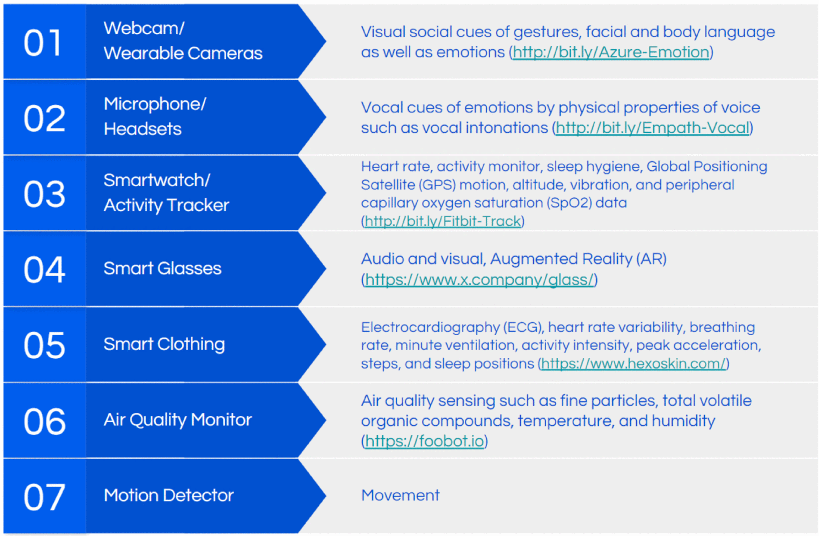
\includegraphics[width = 0.5 \textwidth]{fig01.png}}
\caption{Sensor y tecnología wearable con su respectiva modalidad de información.}
\label{fig1}
\end{figure}

En la sección II describimos conceptos importantes para el mejor entendimiento del presente estudio, en la sección III presentamos algunos casos de aplicación donde destacamos el impacto logrado, en la sección IV presentamos datos del uso de servicios cognitivos para la gestión del conocimiento, en la sección V discutimos posibles nichos de aplicación de servicios cognitivos como parte integral de la gestión del conocimiento, finalmente en la sección VI presentamos nuestras conclusiones.